% !TeX root = ../main.tex

\chapter{系统概要设计}
本章叙述了CI/CD流水线调度系统的设计。
首先介绍了系统的总体设计和架构分层,随后分别叙述系统内各个模块的设计与其之间的连接,
然后后对系统的数据库从概念设计和逻辑设计两方面进行了阐述,最后对本小节内容进行了总结。

\section{系统总体设计}

在对整个CI/CD流水线调度系统进行需求分析后,可以发现本系统的功能业务复杂且对部分服务的横向扩展有着较高需求。
可将本系统拆分为三个微服务,分别为APIServer服务、调度器服务和执行器服务,每个服务下又包含一些子模块。
进行这样服务划分的目的是降低系统间各模块的耦合性,并为不同的模块分配合适的资源,同时也方便不同的模块分别以多节点的方式进行部署。
系统架构图如图~




设计思路+简要介绍

架构图



\section{系统模块设计}
把每个模块讲一下:加入数据流图描述作业数据的流动。

\subsection{CI-Server}

首先是CI-Server模块,系统通过该模块向外部暴露API以供前端/外部接口调用。
用户在前端进行的操作、填写的配置信息等将通过API接口传递给APIServer模块,APIServer模块接收到数据后,会进行相应的业务逻辑处理,如对用户创建的流水线进行合法性校验、对作业数据进行合法性校验等,最后负责将数据落库。
同时,在流水线运行过程中,用户对流水线的手动干预操作,也是先调用接口传递给APIServer模块,然后再由APIServer模块进行一定处理后传递给调度器模块,用户界面与调度器模块完全解耦。

APIServer有以下三种典型服务场景:

当用户通过API接口传入如“取消”、“跳过”、“人工审核通过”等人工干预命令时,APIServer会根据权限模型对用户进行鉴权,如只有流水线的拥有者才有权干预流水线、只有预设的审核人才有权进行人工审核等。
通过鉴权后,APIServer将对人工干预命令进行进一步封装,携带一些额外的信息后,将命令发送给调度器模块,由调度器对流水线的执行进行真正的干预。

当用户通过API接口创建或编辑流水线时,APIServer会对流水线的内容进行解析,并通过序列化器对内容进行合法性校验,然后将流水线以阶段、作业和任务的维度进行分拆,
并将拆解后的流水线数据持久化进数据库。

当用户通过API接口触发流水线时,APIServer将从数据库中获取流水线数据,进行一定封装后发送给调度器模块。
随后,调度器会不断地向APIServer返回流水线的执行信息,以便APIServer实时更新流水线的运行状态。
与此同时,APIServer会接收到前端的轮询请求,用以实时展示给用户。


\subsection{调度器(CI-Master)}

调度器模块是整个系统的核心模块,其中包含状态转移、决策中心与作业管理三个子模块,分别介绍如下:

\subsubsection{状态转移}



\subsubsection{决策中心}

\subsubsection{作业管理}



\subsection{执行器(CI-Runner)}

执行器的设计目的是为了能够稳定高效地执行不同类型的作业,以待执行的作业信息为输入,以作业执行结果为输出,并且支持快速横向扩展,提高作业执行能力。
作业执行器首先需要能够根据自身能够执行的作业类型获取与之相对应的作业。
获取作业之后,能够保证顺利且高效的完成作业执行。
在执行完毕后,将作业状态上报给调度器。
执行器本系统将使用开源的Gitlab Runner,GitLab Runner在Gitlab的CI/CD模块中也扮演执行器的功能,并且与Gitlab主模块使用Http Apis进行通信,本系统中将对这些Http Apis进行抓包,获得这些Api的Url以及出入参后,便可如法炮制地将本系统的调度器接入GitLab Runner。
为了保证系统的稳定性,流水线执行器将部署在Kubernetes中,流水线执行器可以根据当前CI/CD的资源需求自动创建或删除副本(在Kubernetes称作Pod),以适应负载的变化:当系统进入使用高峰期时,系统可以自动创建更多的执行器副本来处理请求,而当负载减少时,多余的副本会被自动删除,从而实现资源的高效利用;
同时,当某个执行器发生故障时,Kubernetes会自动检测到故障,并将受影响的CI/CD负载迁移到其他健康的执行器副本上,避免应用程序中断或停止对外提供服务,提高系统稳定性。


\subsection{消息队列}

本系统调度器与执行器之间的消息交互是借助一个消息队列来完成的,本系统中使用阿里巴巴开发的RocketMq 5.0。
当调度器封装好一个流水线作业运行实例时,调度器将作为消息队列的生产者,将作业运行实例放入队列中;执行器作为消息队列的消费者,将持续消费队列中的消息。
调度器和执行器分别与消息队列进行交互,两者之间解耦,便于后续扩展。

系统引入消息队列的主要目的是实现需求分析中的\nameref{sec:流水线作业合理调度需求}。
首先,消息队列先进先出的特性能够保证执行器有序地消费作业运行实例,避免了程序异步执行带来的作业执行顺序错乱问题,使得作业的执行严格按照调度器预设的顺序执行。
并且,当系统使用高峰期来临,作业量超过了执行器的负载能力时,消息队列承担了缓冲的作用,来不及被消费的作业将按照顺序被堆积在消息队列中,等到执行器处理完当前作业,具备处理能力后,再去消息队列的队头中拉取作业。

调度器、执行器与消息队列之间的时序图如图\ref{fig:消息队列时序图}

\begin{figure}[h]
  \centering
  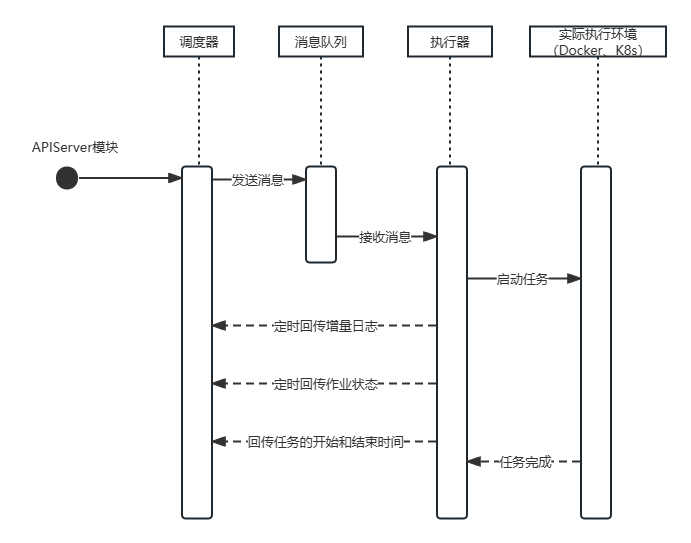
\includegraphics[width=0.8\textwidth]{消息队列时序图.png}
  \caption{调度器、执行器与消息队列间时序图}
  \label{fig:消息队列时序图}
\end{figure}

\subsection{数据存储层}
数据存储层是对本系统中各个数据和文件存储服务的抽象,负责整个系统所有数据的持久化服务。
包括流水线以及其子概念的配置信息、运行记录、Docker镜像、作业执行产物(如编译后压缩产生的tar包等)以及作业运行日志等。


本系统中,使用PostgreSQL存储流水线的配置和运行记录的相关数据,这部分数据属于结构化数据,数据字段和格式较为固定,故采用业界主流的关系型数据库进行存储和管理;
使用Redis存储缓存信息,加快接口的响应速度,提升用户体验;
JFrog Artifactory存储流水线任务执行完成后的执行产物,比如单元测试报告、Docker镜像等;
日志平台建立在 Elastic Search 之上,用于集中记录整个系统的所有运行日志,所有子系统的日志都会传送至该平台进行聚合。
其具体原理与功能与本系统主体功能无关,不再赘述。

上述不同类型的数据及其存储方式总结如表\ref{tab:系统数据存储方式}所示.

\begin{table}[h]
  \centering
  \caption{系统数据存储方式}
  \label{tab:系统数据存储方式}
  \begin{tabular}{clll}
    \toprule
    数据类型 & 主要内容      & 存储方式   & 选型 \\
    \midrule
    结构化数据     & 流水线、阶段、作业与任务的配置信息和运行记录      & 关系型数据库   & PostgreSQL       \\
    缓存数据       & 接口响应数据,提高数据访问速度                   & 键值存储   & Redis       \\
    二进制数据     & 流水线任务执行产物,如单元测试报告、Docker镜像等  & 二进制数据管理系统式   & JFrog Artifactory   \\
    日志数据       & 系统运行日志、流水线作业运行日志等                & 分布式日志系统  & Elastic Search       \\
    \bottomrule
  \end{tabular}
\end{table}

\section{系统功能设计}
功能结构图、自动触发hook序列图



\section{数据模型设计}
这一部分将系统中的数据进行抽象,从实体、属性和关系三个维度设计出系统的数据模型,并基于此完成了对数据表的设计。

本系统的数据实体可以分为两类,一种是配置(Config)相关实体,一种是运行(RunInfo)相关实体。
同时,由于流水线中存在四个不同层级的子概念,所以本系统中可梳理出2×4=8个实体:
流水线配置、阶段配置、作业配置、任务配置、流水线运行记录、阶段运行记录、作业运行记录、任务运行记录。

接下来对实体中的主要属性进行分析。对于配置相关实体,以作业配置实体为例,应主要包含以下几个方面的属性:
基本信息类包括作业id(主键)、作业所属的阶段id(外键)、名称、创建时间、修改时间、作业位于阶段中的位置;
构建信息类包括,包括 Docker 镜像地址、输入环境变量;
执行信息类包括:超时时间、触发类型(自动/人工/定时)、是否启用。
可以得到数据库中作业配置表如表~

对于运行记录相关实体,以作业运行记录为例,应包含以下几个方面的属性:
基本信息类包括作业运行记录id(主键)、作业运行记录所属的阶段运行记录id(外键)、作业运行记录所属的作业id(外键);
触发信息类:触发时间、触发人、触发类型;
运行信息类:开始时间、结束时间、作业状态、赋值后的环境变量;
可以得到数据库中作业运行记录表如表~



其余的流水线配置、阶段配置与任务配置中的属性与作业配置大同小异,此处不再赘述。

对于运行相关实体,以作业运行记录实体为例,应主要包含以下几方面的属性:

最后分析系统内实体之间的关系。一个配置的一次执行即产生了一个运行实例,这与编程语言中“类”和“类对象”的关系类似,
即“运行”是“配置”的实例化,“配置”是“运行”的模板,因此配置与运行是一对多的关系。
同时根据流水线的各个子概念的定义,我们知道有:流水线与阶段是一对多的关系,阶段与作业是一对多的关系,作业与任务是一对多的关系。

结合以上分析,可得出系统的实体-关系图(E-R图)如图~\ref{fig:系统E-R图}:

\begin{figure}[h]
  \centering
  \includegraphics[width=1\textwidth]{ER图.png}
  \caption{系统E-R图}
  \label{fig:系统E-R图}
\end{figure}

\subsection{二级节标题}

\subsubsection{三级节标题}

\paragraph{四级节标题}

\subparagraph{五级节标题}

